\documentclass[a4paper]{article}

\usepackage[brazilian]{babel}
\usepackage[utf8x]{inputenc}
\usepackage[T1]{fontenc}

\usepackage{listings}

%% Useful packages
\usepackage{amsmath}
\usepackage{graphicx}
\usepackage[colorinlistoftodos]{todonotes}
\usepackage[colorlinks=true, allcolors=blue]{hyperref}

\usepackage{mathrsfs}
\usepackage{amssymb}



%opening
\title{Relatório do exercício prático I (E1)}
\author{Daniel Moreira Cestari - 5746193}

\begin{document}

\maketitle

%\section{Introdução}

Basicamente o objetivo deste exercício é gerar os pontos dos bordos, cima, baixo, esquerda e direita, de uma curva fechada fornecida de um arquivo externo.

A geração automática de malhas para domínios com buracos pode gerar pontos fora do domínio, pontos dentro do buraco. Para evitar esse problema, o domínio é artificialmente cortado na hora de especificar seus bordos.

Para esse exercício prático, um arquivo contendo o contorno de um aerofólio é passado como entrada, e como saída o código produzirá um arquivo chamado \textit{output.txt}, caso nenhum nome de saída seja especificado. Desde que o arquivo de entrada da curva contenha uma curva fechada não precisa ser uma curva de um aerofólio. O arquivo de saída trará a especificação dos pontos dos bordos de cima, de baixo, da esquerda e da direita, seguindo a mesma especificação esperada para a geração de malhas dos códigos \textit{elliptic.py} e \textit{transfinita.py}. Esses arquivos foram disponibilizados pelo Professor no formato do \textit{jupyter notebook} e foram convertidos para um código \textit{python}.

O número de pontos da curva passada como entrada determina o número de pontos em cada bordo. Isso acontece pois a curva determina o bordo de cima, e por consequência o número de pontos do bordo de baixo já que ambos precisam ter o mesmo número de pontos. Para os bordos laterais, esquerdo e direito, optou-se por deixar com o mesmo número de pontos que os bordos de cima e de baixo.

O código possui algumas variáveis que podem ser ajustadas para melhorar a geração dos bordos. São valores de \textit{offset} vertical e horizontal (\textit{v\_offset} e \textit{h\_offset}), os valores deixados no código têm os valores \textbf{0,5} e \textbf{1,0}, respectivamente.

O comando para a execução do código é:

\begin{lstlisting}[language=Python]
python ep1.py naca012.txt airfoil.txt
\end{lstlisting}

Utilizando os bordos gerados por esse código como entrada para os códigos \textit{transfinita.py} e \textit{elliptic.py}, ambos foram modificados para receber como entrada o arquivo que farão a leitura dos bordos, é possível gerar as malhas para a curva fechada desejada.

As figuras \ref{fig:swan_transfinita} à \ref{fig:airfoil_elliptic} apresentam as malhas geradas utilizando os códigos explicados acima. Na descrição de cada figura tem o código utilizado para a geração da malha.

\begin{figure}[]
	\centering
	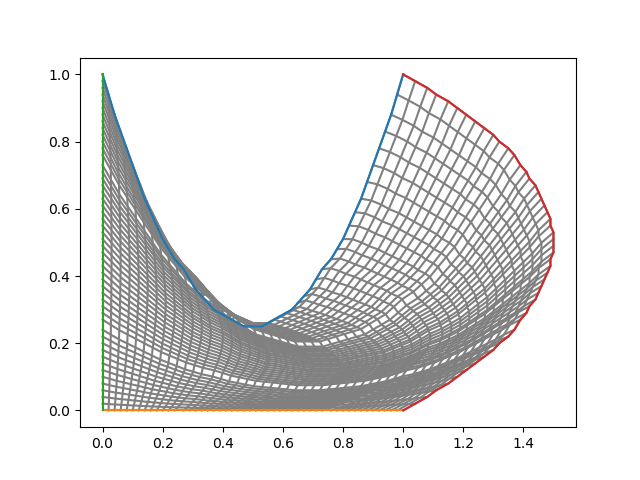
\includegraphics[width=1.0\textwidth]{swan_transfinita.png}
	\label{fig:swan_transfinita} 
	\caption[caption]{Curva \textit{swan} gerada utilizando a interpolação transfinita. \\\hspace{\textwidth} \textit{python transfinita.py swan.txt}}
\end{figure}


\begin{figure}[]
	\centering
	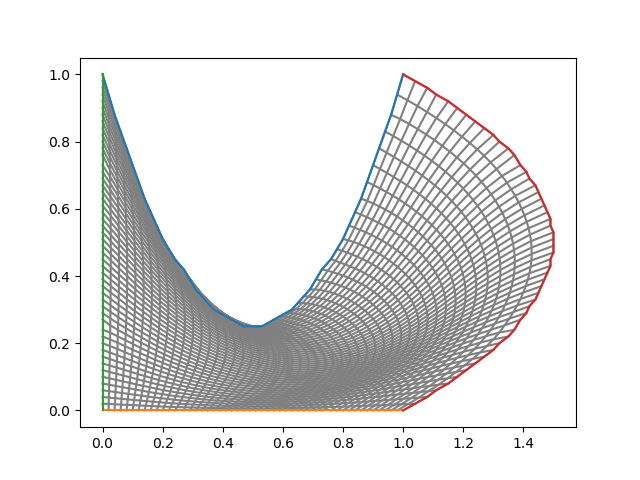
\includegraphics[width=1.0\textwidth]{swan_elliptic.png}
	\label{fig:swan_elliptic} 
	\caption[caption]{Curva \textit{swan} gerada utilizando as equações de Winslow. \\\hspace{\textwidth} \textit{python elliptic.py swan.txt}}
\end{figure}



\begin{figure}[]
	\centering
	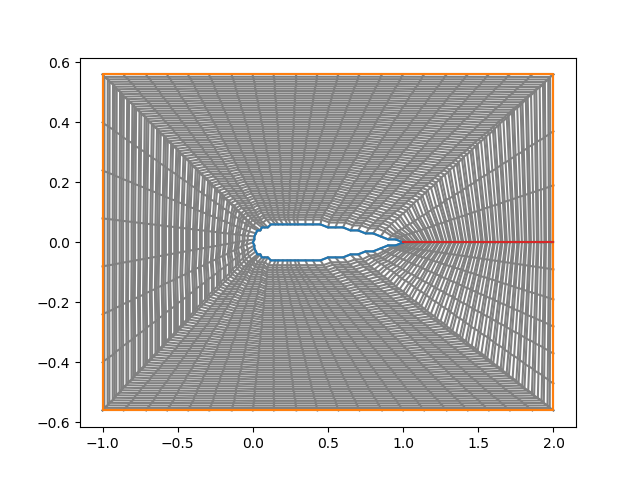
\includegraphics[width=1.0\textwidth]{airfoil_transfinita.png}
	\label{fig:airfoil_transfinita} 
	\caption[caption]{Curva \textit{airfoil} gerada utilizando a interpolação transfinita. \\\hspace{\textwidth} \textit{python transfinita.py airfoil.txt}}
\end{figure}


\begin{figure}[]
	\centering
	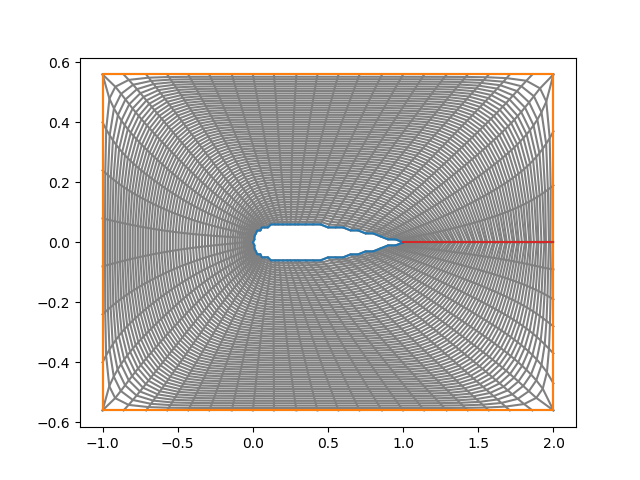
\includegraphics[width=1.0\textwidth]{airfoil_elliptic.png}
	\label{fig:airfoil_elliptic} 
	\caption[caption]{Curva \textit{airfoil} gerada utilizando as equações de Winslow. \\\hspace{\textwidth} \textit{python elliptic.py airfoil.txt}}
\end{figure}


É possível ver que a malha gerada utilizando as equações de Winslow (código \textit{elliptic.py}), que resolvem a equação de Laplace, produzem uma malha muito mais suave que a malha gerada pela interpolação transfinita. Mesmo assim, na curva \textit{swan} essa maneira de gerar malhas mais suaves não foi suficiente para eliminar o problema de gerar pontos fora do domínio. Na Figura \ref{fig:swan_elliptic} é possível ver que há pontos fora, no caso acima, do bordo superior da curva. 

Os códigos gerados e utilizados juntamente com os arquivos contendo os bordos das curvas utilizadas estão disponibilizados no arquivo \textit{zip} que acompanha esse texto.

O próximo trabalho prático abordará conceitos que ajudam a atenuar, ou até mesmo eliminar dependendo dos parâmetros, esse problema.

\end{document}
